Der Aufbau gleicht weitestgehend dem Aufbau der historischen Rutherfordstruung (Abbildung \ref{fig:aufbau}).
Eine $^{241}\symup{Am}$-Quelle befindet sich in einer evakuierbaren Kammer.
Der Träger für die Folien kann in den Strahlengang der Quelle gefahren werden.
Der Detektor ist schwenkbar auf einer Goniometerscheibe montiert und ermöglicht das Messen der Zählraten in Abhängigkeit vom Winkel.
Es liegt ein Oberflächensperrschichtzähler als Detektor vor.
Das Zählwerk ist mit dem Detektor verbunden und kann mit einem Zeitgeber verwendet werden.
Für die Evakuierung steht eine Drehschieberpumpe zur Verfügung.
Hiermit können Drücke bis ca. $\SI{80}{\milli bar}$ erreicht werden.
Zur Abschirmung der äußeren Streustrahlung gibt es einen Deckel, mit dem die Apparatur abgedunkelt werden kann.

\begin{figure}[h!]
  \centering
  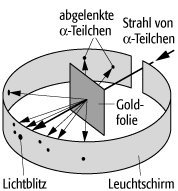
\includegraphics[width=5cm]{images/aufbau_rutherfordstreuung.jpg}
  \caption{Aufbau der historischen Rutherford-Streuung, modifiziert \cite{aufbau}}
  \label{fig:aufbau}
\end{figure}

%Aufbau
%- Quelle
%- Folie
%- Detektor, Winkelverstellbar
%- Vakuumpumpe
%- Zähler mit Taktung (Zeit einstellbar)
%
%Durchführung, Messung der:
%- Dicke der Folie mit Bethe-Bloch (einmal mit Folie, einmal ohne Folie, in Abhängigkeit des Drucks)
%- Winkelabhängigkeit der Rutherfordstreuung einer Folie
%- Z-Abhängigkeit mit verschiedenen Folien
%- große Winkel?
%
